\documentclass[a4paper,10pt]{article}
\usepackage[margin=2.5cm]{geometry}

\usepackage{amssymb,amsmath,amsthm}
\usepackage{color}
\usepackage{enumitem}
\usepackage{dsfont}
\usepackage{bm}


\newtheorem{theorem}{Theorem}
\newtheorem{proposition}{Proposition}
\newtheorem{cor}{Corollary}
\theoremstyle{definition}
\newtheorem{definition}{Definition}
\newtheorem{remark}{Remark}
\newtheorem{example}{Example}
\newtheorem{claim}{Claim}
\newtheorem{lemma}{Lemma}


%%%%%%%%%%%%%%%%%%%%%%%%%%%%%%%%%%%%%%%%%%%%%%%%%%%%%%%%%%%%%%%%%%%%%%%%%%%%%%%
% Algorithms
%%%%%%%%%%%%%%%%%%%%%%%%%%%%%%%%%%%%%%%%%%%%%%%%%%%%%%%%%%%%%%%%%%%%%%%%%%%%%%%

\usepackage{algorithm}
\usepackage{algorithmic}
\usepackage[titlenumbered,ruled,noend,algo2e]{algorithm2e}
\newcommand\mycommfont[1]{\footnotesize\ttfamily\textcolor{blue}{#1}}
\SetCommentSty{mycommfont}
\SetEndCharOfAlgoLine{}


%%%%%%%%%%%%%%%%%%%%%%%%%%%%%%%%%%%%%%%%%%%%%%%%%%%%%%%%%%%%%%%%%%%%%%%%%%%%%%%
% Code
%%%%%%%%%%%%%%%%%%%%%%%%%%%%%%%%%%%%%%%%%%%%%%%%%%%%%%%%%%%%%%%%%%%%%%%%%%%%%%%


\usepackage{fancyvrb}                  % for fancy verbatim
\usepackage{textcomp}
\usepackage[space=true]{accsupp}
% requires the latest version of package accsupp
\newcommand{\copyablespace}{
    \BeginAccSupp{method=hex,unicode,ActualText=00A0}
\ %
    \EndAccSupp{}
}
\usepackage[procnames]{listings}
% \usepackage{setspace} % need for \setstretch{1}
\lstset{%
language   = python,%
 % basicstyle = \ttfamily\setstretch{1},%
basicstyle = \ttfamily,%
columns    = flexible,%
keywordstyle=\color{javared},
firstnumber=100,
frame=shadowbox,
showstringspaces=false,
morekeywords={import,from,class,def,for,while,if,is,in,elif,
else,not,and,or,print,break,continue,return,True,False,None,access,
as,del,except,exec,finally,global,import,lambda,pass,print,raise,try,assert,!=},
keywordstyle={\color{javared}\bfseries},
commentstyle=\color{javagreen}, %vsomb_col white comments
morecomment=[s][\color{javagreen}]{"""}{"""},
upquote=true,
%% style for number
numbers=none,
resetmargins=true,
xleftmargin=10pt,
linewidth= \linewidth,
numberstyle=\tiny,
stepnumber=1,
numbersep=8pt, %
frame=shadowbox,
rulesepcolor=\color{black},
procnamekeys={def,class},
procnamestyle=\color{oneblue}\textbf,
literate={á}{{\'a}}1
{à}{{\`a }}1
{ã}{{\~a}}1
{é}{{\'e}}1
{ê}{{\^e}}1
{è}{{\`e}}1
{í}{{\'i}}1
{î}{{\^i}}1
{ó}{{\'o}}1
{õ}{{\~o}}1
{ô}{{\^o}}1
{ú}{{\'u}}1
{ü}{{\"u}}1
{ç}{{\c{c}}}1
}


\usepackage{times} % use Times

\usepackage{../sty/shortcuts_js} % possibly adapted from https://github.com/josephsalmon/OrganizationFiles/sty/shortcuts_js.sty

%%%%%%%%%%%%%%%%%%%%%%%%%%%%%%%%%%%%%%%%%%%%%%%%%%%%%%%%%%%%%%%%%%%%%%%%%%%%%%%
% IMAGES
%%%%%%%%%%%%%%%%%%%%%%%%%%%%%%%%%%%%%%%%%%%%%%%%%%%%%%%%%%%%%%%%%%%%%%%%%%%%%%%

% Use prebuiltimages/ for images extracted from code (e.g. python)
% or to share images built from a software not available by the whole team (say matlab .fig, or inskcape .svg).
% .svg files should be stored in dir srcimages/ and built from moosetex if needed:
% https://www.charles-deledalle.fr/pages/moosetex.php
% NEVER (GIT) versions files in images/ : only prebuiltimages/ & srcimages/ !

\usepackage{graphicx} % For figures
\graphicspath{{images/}, {prebuiltimages/}}
\usepackage{subcaption}


%%%%%%%%%%%%%%%%%%%%%%%%%%%%%%%%%%%%%%%%%%%%%%%%%%%%%%%%%%%%%%%%%%%%%%%%%%%%%%%
% For citations
%%%%%%%%%%%%%%%%%%%%%%%%%%%%%%%%%%%%%%%%%%%%%%%%%%%%%%%%%%%%%%%%%%%%%%%%%%%%%%%

\usepackage[authoryear]{natbib}
\usepackage{cleveref} % mandatory for no pbs with hyperlinks theorem etc...
\crefformat{equation}{Eq.~(#2#1#3)} % format for equations
\Crefformat{equation}{Equation~(#2#1#3)} % format for equations


%%%%%%%%%%%%%%%%%%%%%%%%%%%%%%%%%%%%%%%%%%%%%%%%%%%%%%%%%%%%%%%%%%%%%%%%%%%%%%%
% Header and document start
%%%%%%%%%%%%%%%%%%%%%%%%%%%%%%%%%%%%%%%%%%%%%%%%%%%%%%%%%%%%%%%%%%%%%%%%%%%%%%%


\author{Rudolf Römisch}
\title{Outlier-robust estimation of a sparse linear model using $l_1$-penalized Huber's M-estimator}

\begin{document}

\maketitle

\vskip 0.3in

\begin{abstract}
Here we discuss linear models of estimating coefficients of p-dimensional s-sparse vectors with Gaussian design and additive noise. We consider the case of contaminated labels by at most o adversarial outliers. With that we prove that the $l_1$-penalized Huber's M-estimator based on n samples attains the optimal rate of convergence $(s/n)^{1/2}$ +$(o/n)$, up to a logarithmic factor.
For more general design matrices, our results highlight the importance of two properties: the transfer principle and the incoherence property. These properties with suitable constants are shown to yield the optimal rates, up to log-factors, of robust estimation with adversarial contamination.
\end{abstract}


\section{Introduction}\ \\
The paper deals with the question if it is possible to attain optimal rates of estimation in outlier-robust sparse regression using penalized empirical risk minimization (PERM) with convex loss and convex penalties and compares past literature. They emphasize that there is a certain direction the research is going and not in a positive way to answer the question.\\

Since no method based on empirical loss minimization with convex loss and convex penalty can lead to consistent support recovery, some authors advocate for robustifying the $l_1$-penalized least-squares estimators by replacing usual scalar products by their trimmed counterparts.
Furthermore other work established that in the multivariate Gaussian model subject to Huber's contamination, coordinatewise median - which is the ERM for the $l_1$-loss - is sub-optimal.
In this report we consider the $l_1$-penalized empirical risk minimizer based on Huber's loss which is shown to be minimax-rate-optimal, up to possible logarithmic factors.
It is important to mention that in the most general case the results are not valid. We put some assumpution to the design matrix and the response. The design matrix satisfies some incoherence condition and only the response is subject to contamination.\\
The incoherence condition is shown to be satisfied by the Gaussian design with a covariance matrix that has bounded and bounded away from zero diagonal entries.
We choose this simple setting in order to get to the main result:\\
for properly chosen convex loss and convex penalty functions, the PERM is minimax-rate-optimal in sparse linear regression with adversarially corrupted labels.

\section{Model}\ \\
First we consider the model with "clean" data where
	$\mathcal{D}_n$° = $\{(\boldmath{X}_i, y_i$°$); i = 1,...,n \}$ be the independed identical distributed (i.i.d.) feature-label pairs. We get to the standard linear model:
\begin{equation}
	y_i = \bold{X}_i^T\beta^* + \xi_i, \quad i=1,...,n,
\end{equation}
where $\boldmath{X}_i \in \mathbb{R}^p$ are Gaussian with zero mean and covariance matrix $\Sigma$,
$y_i^{\circ}$ are the responses defined by the linear model above,
and $\xi_i ~ \mathcal{N}(0,\sigma^2)$ is the random noise which is independent of $\boldmath{X}_i$.
But instead of having access to the "clean" data, we are limited of the contaminated version which is $\mathcal{D}_n$ = $\{(\boldmath{X}_i, y_i); i = 1,...,n \}$. A small number $o \in \{1,...,n\}$ of labels $y_i^{\circ}$ are replaced by an arbitrary value.
Now we are setting $\theta^*_i = (y_i - y_i^{\circ})/\sqrt{n}$ and using matrix-vector notation to get to the contaminated model:
\begin{equation}
	\bold{Y} = \bold{X\beta^*} + \sqrt{n} \bold{\theta^*} + \bold{\xi}.
\end{equation}
Here we have $\boldmath{X} = [\boldmath{X}_1^T;...;\boldmath{X}^T_n]$ as the $n\times p$ design matrix, $\boldmath{Y}$ = $(y_1,...,y_n)^T$ as the response vector, $ \boldsymbol{\theta^*} = (\theta^*_1,...,\theta^*_n)^T$ as the contamination vector and $\boldsymbol{\xi} = (\xi_1,...,\xi_n)^T$ as the noise vector.

The goal is to estimate the vector $\boldsymbol{\beta}^* \in \mathbb{R}^p$. The dimension p is assumed to be large, possibly larger than n but, for some small value $s \in \{1,...,p\}$, the vector $\boldsymbol{\beta}^*$ is assumed to be s-sparse: $||\boldsymbol{\beta}^*||_0 = Card\{j:\beta^* \neq 0\} \leq s$. If we have access to the clean data $\mathcal{D}_n$° and measure the quality of an estimator $\hat{\beta}$ by the Mahalanobis norm $||\Sigma^{1/2}(\hat{\beta}- \beta^*)||_2$, the optimal rate is 
\begin{equation}
	r^{\circ}(n,p,s) = \sigma(\frac{slog(p/s)}{n})^{1/2}.
\end{equation}

Whereas in the outlier-contaminated setting where we do not have access to the "clean" data, the minimax-optimal-rate takes the form:
\begin{equation}
	r(n,p,s,o) = \sigma(\frac{slog(p/s)}{n})^{1/2} + \frac{\sigma o}{n}.
\end{equation}

The assumption that only a small number o of labels are contaminated by outliers implies that the vector $\boldsymbol{\theta}^*$ in (1) is o-sparse. In order to take advantage of sparsity of both $\boldsymbol{\beta}^*$ and $\boldsymbol{\theta}^*$ while ensuring computational tractability of the resulting estimator, a natural approach is to use some version of the $l_1$-penalized ERM. This corredsponds to defining:

\begin{equation}
	\hat{\bold{\beta}} \in arg
	\min\limits_{\bold{\beta}\in
	\mathbb{R}^p} \min\limits_{\bold{\theta}\in
	\mathbb{R}^n}\{\frac{1}{2n} ||\bold{Y} - \boldsymbol{X^T\beta} - \sqrt{n}\boldsymbol{\theta}||_2^2 + \lambda_s ||\boldsymbol{\beta}||_1 + \lambda_o||\boldsymbol{\theta}||_1\},
\end{equation}
where $\lambda_s, \lambda_o > 0$ are tuning parameters. The best known rate for this type of estimator is:
\begin{equation}
	\sigma (\frac{slog(p)}{n}^{1/2}) + \sigma(\frac{0}{n})^{1/2},
\end{equation}
under some restrictions on (n,p,s,o). When we compare (6) to (4) we can see that (6) is sup-optimal and the ratio of the two rates may be as large as $(n/o)^{1/2}$. \\
The very goal is to show that this sub-optimality is not an intrinsic property of the estimator (5), but rather an artefact of previous proof techniques. By using a refined argument, we prove that $\boldsymbol{\hat{\beta}}$ defined by (5) does attain the optimal rate under very mild assumptions.
Now we refer to $\boldsymbol{\hat{\beta}}$ as $l_1$-penalized Huber's M-estimator. The rationale for this term is that the minimization with respect to $\boldsymbol{\theta}$ in (5) can be done explicitly. It yields:

\begin{equation}
		\boldsymbol{\hat{\beta}} \in arg \min\limits_{\bold{\beta}\in
		\mathbb{R}^p} \{ \lambda_o^2 \sum_{i = 1}^{n}\Phi (\frac{y_i - \bold{X}^T_i \bold{\beta}}{\lambda_o \sqrt{n}}) + \lambda_s||\bold{\beta}||_1\}
\end{equation}
where $\Phi:\mathbb{R} \rightarrow \mathbb{R}$ is Huber's function defined by $\Phi (u) = (1/2)u^2 \vee (|u|-1/2)$.
Next we establish a risk bound for a general design matrix $\bold{X}$ not necessarily formed by Gaussian vectors. With that we prove the rate-optimality of the estimator $\boldsymbol{\hat{\beta}}$.


\newpage
\section{Risk bound for the $l_1$-penalized Huber’s M-estimator}\ \\

In this part we bring sufficient conditions on the design matrix that allow for rate-optimal risk bounds for the estimator $\boldsymbol{\hat{\beta}}$ defined by (5) or (7). There are two qualitative conditions that can be seen to be necessary: the restricted invertibility and incoherence. Even when there is no contamination, the number of outliers is known to be $o=0$, the matrix $\bold{X}$ has to satisfy a restricted invertibility condition in order that the Lasso estimator (5) does achieve the optimal rate $\sigma\sqrt{(s/n)log(p/s)}$. But also in the case where $n=p$ and $\bold{X} = \sqrt{n}\bold{I}_n$, even in the extremely favorable situation where the noise $\boldsymbol{\xi}$ is zero, the only identifiable vector is $\boldsymbol{\beta}^* + \boldsymbol{\theta}^*$. Therefore, it is impossible to consistently estimate $\boldsymbol{\beta}^*$ when the design matrix $\bold{X}$ is aligned with the identity matrix $\bold{I}_n$ or close to be so.\\

The next definition formalizes what we call restricted invertibility and incoherence by introducing three notions: the transfer principle, the incoherence property and the augmented transfer principle. These are a crucial part in the robust estimation by $l_1$-penalized least squares.

\begin{definition}
	Let $ \bold{Z} \in \mathbb{R}^{nxp} $ be a (random) matrix and $ \Sigma \in \mathbb{R}^{pxp} $. We use notation $ \bold{Z}^{(n)} = \bold{Z}/\sqrt{n}$.\\
	\begin{itemize}
		\item (i) We say that $\bold{Z}$ satisfies the transfer principle with $a_1 \in (0,1)$ and $a_2 \in (0,\infty)$, denoted by $TP_{\Sigma}(a_1;a_2)$, if for all $\bold{v} \in \mathbb{R}^p$,
		\begin{equation}
			||\bold{Z}^{(n)}||_2 \geq a_1 ||\Sigma^{1/2}\bold{v}||_2 - a_2||\bold{v}||_1
		\end{equation}
		
		\item (ii) We say that $\bold{Z}$ satisfies the incoherence property $IP_{\Sigma}(b_1;b_2;b_3)$ for some positive numbers $b_1, b_2 and b_3$, if for all $[v;u] \in \mathbb{R}^{p+n}$,
		\begin{equation}
			|u^T Z^{(n)}v| \leq b_1||\Sigma^{1/2}v||_2||u||_2 + b_2||v||_1||u||_2 + b_3||\Sigma^{1/2}v||_2||u||_1.
		\end{equation}
		\item (iii) We say that $ \bold{Z} $ satisfies the augmented transfer principle $ATP_{\Sigma}(c_1;c_2;c_3)$ for some positive numbers $c_1, c_2 and c_3$, if for all $[v;u]\in \mathbb{R}^{p+n}$,
		\begin{equation}
			||\bold{Z}^{(n)}v+u||_2 \geq c_1||[\Sigma^{1/2}v;u]||_2 - c_2||v||_1 - c_3||u||_1.
		\end{equation}
	\end{itemize}
	
	These three properties are inter-related and related to extreme singular values of the matrix $\bold{Z}^{(n)}$.
	
	\begin{itemize}
		\item (P1) If Z satisfies $ATP_{\Sigma}(c_1;c_2;c_3)$ then it also satisfies $TP_{\Sigma}(c_1;c_2)$.
		\item (P2) If Z satisfies $TP_{\Sigma}(a_1;a_2)$ and $IP_{\Sigma}(b_1;b_2;b_3)$ then it also satisfies $ATP_{\Sigma}(c_1;c_2;c_3)$ with $c^2_1 = a_1^2 - b_1 - \alpha^2$, $c_2 = a_2 + 2b_2/\alpha$ and $c_3 = 2b_3/\alpha$ for any positive $\alpha < \sqrt{a^2_1 - b_1}$.
		\item (P3) If Z satisfies $IP_{\Sigma}(b_1;b_2;b_3)$, then it also satisfies $IP_{\Sigma}(0;b_2;b_1+b_3)$.
		\item (P4) Any matrix Z satisfies $TP_I(s_p(Z^{(n)});0)$, and $IP_I(s_1(Z^{(n)});0;0)$, where $s_p(Z^{(n)})$ and $s_1(Z^{(n)})$ are, respectively, the p-th largest and the largest singular values of $\bold{Z}^{(n)}$.
	\end{itemize}
	
\end{definition}


Now to state the theorem below we consider the simplified setting in which $\lambda_s = \lambda_o = \lambda$. Also we normalize the columns of the matrix $\bold{X}$ so that their Euclidean norm is of the order $\sqrt{n}$.
For our following consideration we recall that a matrix $\Sigma$ is said to satisfy the restricted eigenvalue condition RE($s,c_0$) with some constant $\varkappa >0$, if
\begin{equation*}
	||\Sigma^{1/2}\bold{v}|| \geq \varkappa ||\bold{v}_J||_2
\end{equation*}
for any vector $\bold{v}\in \mathbb{R}^p$ and any set $J \subset \{1,...,p\}$ such that $Card(J) = \leq s$ and $||\bold{v}_{J^c}||_1 \leq c_0||\bold{v}_J||_1$.

\begin{theorem}\ \\
	Let $\Sigma$ satisfy the RE(s,5) condition with constant $\varkappa > 0$. Let $b_1,b_2,b_3, c_1, c_2, c_3$ be some positive real numbers such that $\bold{X}$ satisfies the $IP_{\Sigma}(0;b_2;b_3)$ and the $ATP_{\Sigma}(c_1;c_2;c_3)$. Assume that for some $\delta \in (0,1)$, the tuning parameter $\lambda$ satisfies
	\begin{equation*}
		\lambda \sqrt{n} \leq \sqrt{8 log(n/\delta)} \bigvee (\max\limits_{j = 1,...,p}||\bold{X}_{\bullet, j}^{(n)}||_2)\sqrt{8log(p/\delta)}.
	\end{equation*}
	If the sparsity s and the number of outliers o satisfy the condition
	\begin{equation*}
		\frac{s}{\varkappa^2} + o \leq \frac{c_1^2}{400(c_2 \vee c_3 \vee 5b_2/c_1)},
	\end{equation*}
	then, with probability at least $1-2\delta$, we have
	\begin{equation*}
		||\bold{\Sigma}^{1/2}(\hat{\beta}- \beta^*)||_2 \leq \frac{24\lambda}{c_1^2}(\frac{2c_2}{
			c_1} \bigvee \frac{b_3}{c_1^2}) (\frac{s}{\varkappa^2} + 7o) + \frac{5\lambda\sqrt{s}}{6c_1^2\varkappa}.
	\end{equation*}
\end{theorem}

For the case of a Gaussian design considered in the next section, $c_1$ is of order $1$ while $b_2,b_3,c_2,c_3$ are of order $n^{-1/2}$, up to a logarithmic factor in p, n and $1/\delta$. Here $\delta$ is an upper bound on the probability that the Gaussian matrix $\bold{X}$ does not satisfy either $ATP_{\Sigma}$ or $IP_{\Sigma}$. This will make the theorem easier to parse.


	
\section{Case of Gaussian Design}\ \\	
	
	The main result in the section before shows that if the design matrix satisfies the transfer principle and the incoherence property with suitable constants, then the $l_1$-penalized Huber's M-estimator achieves the optimal rate under adversarial contamination. As a concrete example of a design matrix for which the conditions are satisfied, we consider the case of correlated Gaussian design.\\
	We will introduce some assumptions to get an easier access to the results. With a more extensive research the assumptions can be more general but the proof might get more complicated.
	First we will allow the covariance matrix to have a non degenerate null space. Also we assume that the n rows of the matrix $\bold{X}$ are independently drawn from the Gaussian distribution $\mathcal{N}_p(\bold{0},\boldsymbol{\Sigma})$ with a covariance matrix $\boldsymbol{\Sigma}$ satisfying the RE($s,5$) condition. Furthermore all diagonal entries of $\boldsymbol{\Sigma})$ are equal to 1. Now we get the following theorem:
	
	
	\begin{theorem}\ \\
		Let $\delta \in (0, 1/7)$ be a tolerance level and $n \leq 100$. For every positive semi-definite matrix $\bold{\Sigma}$ with all the diagonal entries bounded by one, with probability at least $1-2\delta$, the matrix $\bold{X}$ satisfies the $TP_{\Sigma}(b_1,b_2,b_3)$ and the $ATP_{\Sigma}(c_1,c_2,c_3)$ with constants
		\begin{equation}
			a_1 = 1-\frac{4.3+\sqrt{2log(9/\delta)}}{\sqrt{n}}, \quad a_2=b_2=1.2\sqrt{\frac{2log(p)}{n}},
		\end{equation}
		
		\begin{equation}
			b_1 = \frac{4.8\sqrt{2} + \sqrt{2log(81/\delta)}}{\sqrt{n}}, \quad b_3=1.2\sqrt{\frac{2log(n)}{n}},
		\end{equation}
		
		\begin{equation}
			c_1=\frac{3}{4} - \frac{17.5 + 9.6\sqrt{2log(2/\delta)}}{\sqrt{n}}, \quad c_2 = 3.6 \sqrt{\frac{2log(p)}{n}}, \quad c_3=2.4\sqrt{\frac{2log(n)}{n}}.
		\end{equation}
		
	\end{theorem}

For the case of imposing even more restrictions on $n,p,s$ and $o$ we get the following theorem:

	\begin{theorem}\ \\
		There exist universal positive constants $d_1, d_2, d_3$ such that if
		\begin{equation}
		 	\frac{s log(p)}{\varkappa^2} + o log(n) \leq d_1n \quad and \quad 1/7 \geq \delta \geq 2e^{-d_2n}
		\end{equation}
		then, with probability at least $1-4\delta$, $l_1$-penalized Huber's M-estimator with $\lambda^2_sn = 9\sigma^2 log (p/\delta)$ and $\lambda^2_on = 8\sigma^2 log (n/\delta)$ satisfies
		\begin{equation*}
			||\bold{\Sigma}^{1/2}(\hat{\beta}-\beta^*)||_2 \leq d_3 \sigma \Big\{ (\frac{slog(p/\delta)}{n\varkappa^2})^{1/2} + \frac{olog(n/\delta)}{n} \Big\}.
		\end{equation*}
	\end{theorem}

This result is compared to previous work an improvement in the rate. Not only in terms of its dependence on the proportion of outliers, o/n, but also in terms of the condition number $\varkappa$, which is now completely decoupled from o in the risk bound.\\
While the main focus is on the high dimensional situation in which p can be larger than n, it also applies to the case of small dimensional dense vectors, that means when s=p is significantly smaller than n. By comparison to previous and similar work our Theorem (3) 
implies that the error of the $l_1$-penalized Huber's estimator goes to zero at the faster rate $\sigma^2 \{(s/n)+(o/n)^2\}$. Even further, through Theorem (3)
 some can deduce that as soon as the number of outliers satisfies 
 $o=o(\sqrt{sn/\varkappa^2})$, the rate of convergence remains the same as in the outlier-free setting.

\newpage

\section{Extensions}\ \\
With the previous sections, it is easy to see that there is room for further investigations. Mainly in the direction of even more general cases.

\subsection{Contaminated Design}\ \\
The first case would be extended case of not only the contaminated response vector but also contaminated features. In such a setting, we would set
\begin{equation*}
	\theta_i^* = (y_i - \bold{X}^T_i\boldsymbol{\beta}^* - \xi_i)/\sqrt{n}
\end{equation*}
and recover exactly the same model as in (2).\\
The important difference as compared to the setting investigated in previous section is that it is not reasonable anymore to assume that the feature vectors {$\bold{X}_i:i\in O$} are i.i.d. Gaussian. In the adversarial setting, they may even be correlated with the noise vector $\boldsymbol{\xi}$. It is then natural to remove all the observations for which $max_j||\bold{X}_{ij} > \sqrt{2log(np/\delta)}$ and to assume, that the $l_1$-penalized Huber estimator is applied to data for which $max_{ij}|\bold{X}_{ij}| \leq \sqrt{2log(np/\delta)}$.
Taking into account the transfer principle and the incoherence property we obtain the following rate:
\begin{equation}
	||\bold{\Sigma}^{1/2}(\hat{\beta}-\beta^*)||_2 =\sigma O \Big\{ \sqrt{\frac{s}{n}} + \frac{\sqrt{o^3}}{n} \Big\}.
\end{equation}
This rate of convergence appears to be slower but improvable. Also the estimator $\boldsymbol{\hat{\beta}}$ has the advantage of being independent of the covariance matrix $\boldsymbol{\Sigma}$ and on the sparsity s.

\subsection{Sub-Gaussian Design}\ \\
The second Theorem makes use of some inequalities which are specific to the Gaussian distribution. So further research would question if the rate $\sigma \Big\{ (\frac{slog(p/s)}{n})^{1/2} + \frac{0}{n} \Big\}$ can be obtained for more general design distributions.

\subsection{Heavier tailed Noise Distributions}\ \\
For simplicity, we assumed that the random variables $\xi_i$ are drawn from a Gaussian distribution. All the results extend to the case of sub-Gaussian noise. So we only need to control tail probabilites of the random variable $||\bold{X}^T\boldsymbol{\xi}||_{\infty}$ and $||\boldsymbol{\xi}||_{\infty}$, which can be done by standard methods. So it should be possible to extend the results beyond sub-Gaussian noise, assuming type of heavy-tailed distributions. The rational behind this is that any random variable $\xi$ can be written as a sum of sub-Gaussian variable $\xi^{noise}$ and a "sparse" variable $\xi^{out}$. By "sparse" we mean that $\xi^{out}$ takes the value 0 with high probability. The random noise terms $\xi_i^{out}$ can be merged with $\theta_i$ and considered as outliers. Maybe this approach can establish a connection between two types of robustness: to outliers and heavy tails.


\section{Numerical Illustration}

To see the obtained theoretical result we will consider an illustration performed with the variables as a numerical result. The following plot has n = 1000 and p = 100 for three different levels of sparsity s = 5,15,25. The noise variance was set to 1 and $\boldsymbol{\beta}^*$ was set to have its first s non-zero coordinates equal to 10. Each corrupted response coordinate was $\theta^*_j = 10$. The fraction $\epsilon = o/n$ of outliers was ranging between 0 and 0.25 with a step size of 5 for the number of outliers o is used.
\centering
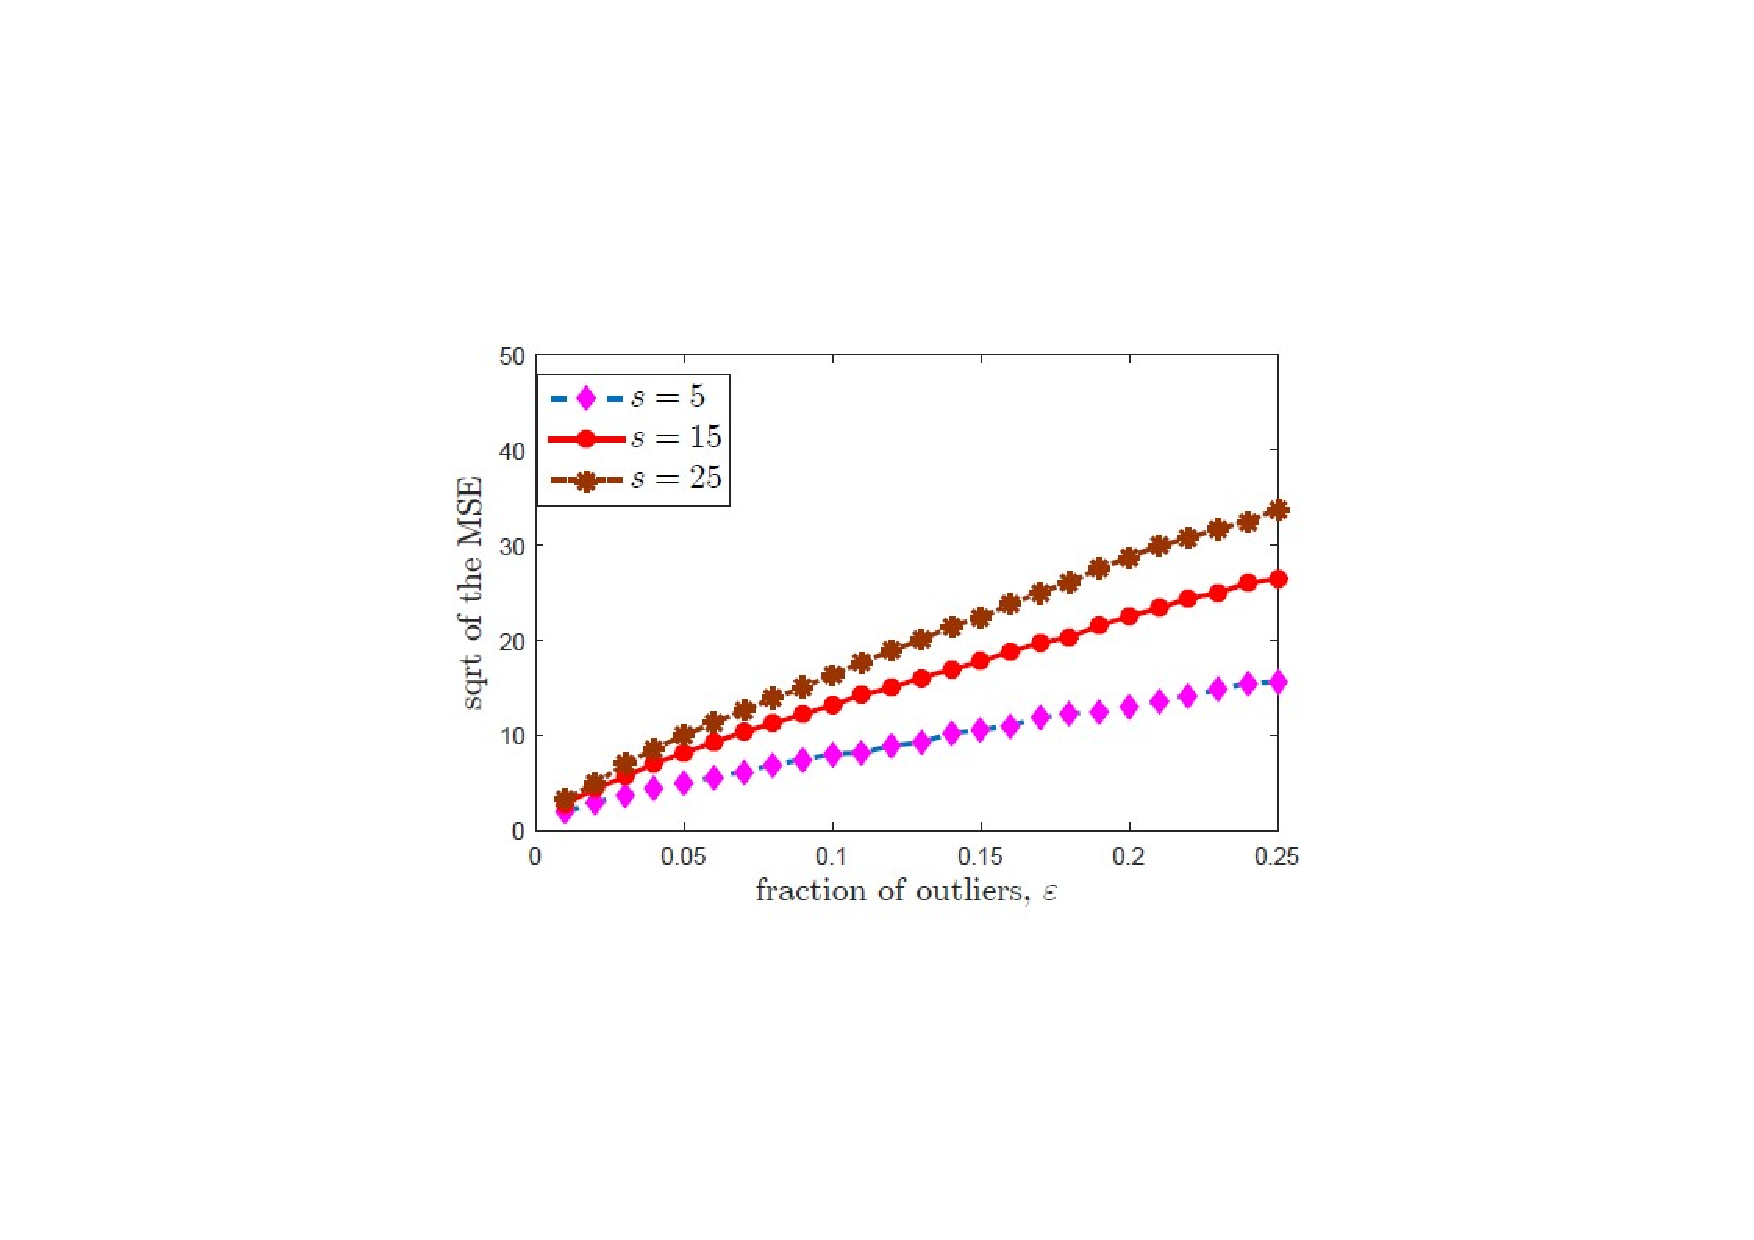
\includegraphics{numerical_illustration.pdf}



\section{Conclusion}\ \\

In this work we described the overall setting and the goal behind it. We introduced the standard case and with that the possible case of sparse and contaminated vectors. Through the third section, which is the heart of this work, we established risk bounds for that we can prove the optimal rate. Then in the next section we embedded the work in the Gaussian Design.
We have seen the rate-optimality - up to logarithmic terms that can be avoided - of $l_1$-penalized Huber's M-estimator in the setting of robust linear regression with adversarial contamination. 
Additionally in finding an improved rate of convergence, we also relaxed the assumptions on the design. Furthermore the outlined possible extensions are promising for future research.





\end{document}
